\section{Calibrazione}
	L'obiettivo della calibrazione è misurare lo "zero" del goniometro e il passo del reticolo di diffrazione.
	
	Si è montata la lampada al mercurio e si è proceduto come nella parte precedente:
	si è rimosso il reticolo e si sono allineate sorgente, fessura di ingresso del telescopio di raccolta
	ed il reticolo a croce del telescopio di osservazione.
	
	Abbiamo assunto la lettura del goniometro
	$\alpha_0$ quale zero di riferimento per le successive misure.
	Essendo tale misura basilare per le osservazioni successive la stessa è stata ripetuta da ogni membro del gruppo,
	ottenendo la stima finale di $\alpha_0 = \ang{171;21; } \pm 3' $.
	
	Si è quindi reinserito il reticolo ad un angolo $\sim \ang{60}$
	tra normale e fascio incidente.

	Per misurare il passo del reticolo si è misurato l'angolo di riflessione (ordine zero) della della sorgente sul reticolo e successivamente la riga di emissione principale del mercurio (verde) al 
	primo e secondo ordine di diffrazione. La lunghezza d'onda è nota essere $\lambda = \SI{546.074}{\nano\meter}$,
	ottenendo rispettivamente $\alpha_0=\ang{58;24;} \pm 6'$, $\alpha_1=\ang{105;55}\pm 6"$ e $\alpha_1=\ang{144;32}\pm 6"$.
	
	Essendo nota la relazione:
	\smallskip
	\begin{equation*}
	d(sin (\alpha_i) - sin (\alpha_d) = m \lambda\qquad \text{con}\qquad \theta_i=\frac{1}{2}(\pi- \alpha_0)\qquad \alpha_i=(\pi- \theta_1-\alpha_m)
	\end{equation*}
	Dove per gli angoli si è seguita la notazione usata in \figurename{ \ref{fig:angoli}}.
	\bigskip
	\begin{figure} [H]
		\centering
		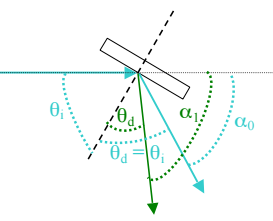
\includegraphics[width=0.4\textwidth]{../FIgs-tabs/angoli.png}
		\caption{Schema della convenzioni degli angoli impiegata.}
		\label{fig:angoli}
	\end{figure}
	\smallskip

È quindi possibile ricavare il passo reticolare $d=	\SI{84.27 \pm 0.08}{\micro\meter}$.

\section{Misura della costante di Rydberg}
	Si è sostituita la lampada al mercurio con quella all'idrogeno e si è proceduto alla misura delle righe osservabili e dell'ordine zero di riflessione.
	
	Le misure effettuate e le lunghezza d'onda ricavate sono riportate di seguito:
	\smallskip
	\begin{table}[H]
	\centering
		\begin{tabular}{c|c|c|c}
			riga & ordine & $\alpha _{m}$ & $\lambda \;\text{(nm)}$ \\
		\hline
		& $ 0 $ &$\ang{58;17;} \pm 6' $ &\\
		\hline
		blu (\SI{434.1}{\nano\meter})& $ 1 $ &$\ang{97;54;30} \pm 6' $ & $430.7 \pm 0.9$\\
		\hline
		 & $ 2$ & $\ang{128;12;} \pm 6' $ &$434.4 \pm 0.6$\\
		\hline
		verde (\SI{486.1}{\nano\meter}) & $ 1$ & $\ang{101;42;} \pm 6' $ &$483.5 \pm 1.0$\\
		\hline
		 &$ 2$ & $\ang{135;37;30} \pm 6' $&$487.6 \pm 0.6$ \\
		\hline
		rosso (\SI{656.3}{\nano\meter})&$1$ & $\ang{113;36;30} \pm 6' $ &$654.6 \pm 1.1$\\
		\end{tabular}
	\end{table}
	\smallskip

	Impiegando la nota relazione:
	\smallskip
	\begin{equation*}\label{eq:ryd}
	\frac{1}{\lambda}=R\;\biggl(\frac{1}{{n_1}^2}-\frac{1}{{n_2}^2}\biggr)
	\end{equation*}
	\smallskip
si può eseguire un fit lineare per la costante di Rydberg, ottenendo un valore di $R= \SI{1.0979\pm0.0008e7}{\meter^{-1}}$ che è in ottimo accordo con il valore noto di $R= \SI{1.0974e7}{\meter^{-1}}$.

Di seguito è riportato il grafico del fit eseguito.

	\begin{figure} [H]
		\centering
		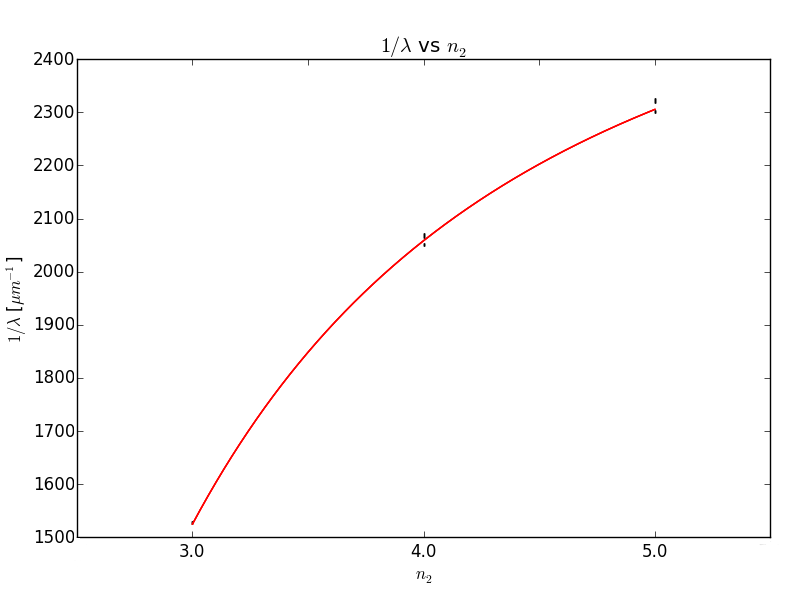
\includegraphics[width=0.7\textwidth]{../FIgs-tabs/fit_R.png}
		\caption{Fit della costante di Rydberg}
	\end{figure}

\section{Stima della risoluzione dello spettroscopio}
	Per effettuare una stima della sensibilità dello
	spettroscopio si è montata come sorgente la 
	lampada al sodio e si è misurata la posizione angolare delle righe del doppietto giallo
	del sodio, ottenendo $$\alpha_0= \ang{57;57;} \pm 6'}
	\text{, }\alpha_1=	\ang{108;56;}\pm 6' \text{ e } \Delta\alpha=2' \pm 1'$$
rispettivamente l'angolo di riflessione, l'angolo della prima riga del doppietto e la distanza angolare dalla seconda.
Per la lunghezza d'onda delle due righe si ottiene:
	$$\lambda_1= \SI{589.8 \pm 1.1}{\nano\meter}\text{ e } \lambda_2=  \SI{590.3 \pm 1.0}{\nano\meter}$$
	Tali misure risultano in accordo con 
	la misura effettuata con l'apparato della prima parte e con il valore atteso di $\lambda_1^{exp}= \SI{589.0}{\nano\meter}\text{ e } \lambda_2^{exp}=  \SI{589.9}{\nano\meter}$.
		La larghezza del doppietto misurata risulta essere $\Delta 	\lambda=\SI{0.48 \pm 0.24}{\nano\meter}$ che è compatibile con quella attesa $\Delta 	\lambda^{exp}=\SI{0.6}{\nano\meter}$.